\documentclass{standalone}
\usepackage{tikz}
\begin{document}

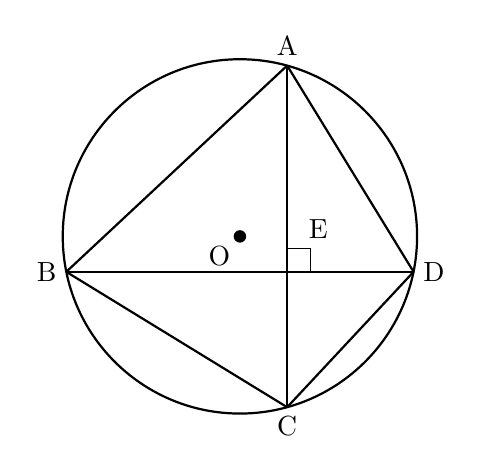
\begin{tikzpicture}[scale=1.5]
    % বৃত্তের ব্যাসার্ধ নির্ধারণ
    \def\r{1.5}
    
    % কেন্দ্র ও বৃত্ত অঙ্কন
    \coordinate (O) at (0,0);
    \draw[thick] (O) circle (\r);
    \fill (O) circle (1.5pt); % কেন্দ্র বিন্দু
    \node at (O) [below left] {O}; % কেন্দ্রের লেবেল
    
    % জ্যা-দ্বয়ের ছেদবিন্দু E (কেন্দ্রের একটু নিচে ও ডানে)
    \coordinate (E) at (0.5, -0.1);
    \node at (E) [above right] {E};
    
    % জ্যা AC অঙ্কন (উল্লম্ব রেখা যা E বিন্দু দিয়ে যায়)
    % x^2 + y^2 = r^2 সূত্র ব্যবহার করে ছেদবিন্দু বের করা হয়েছে
    \coordinate (A) at (0.4, 1.446);
    \coordinate (C) at (0.4, -1.446);
    \draw[thick] (A) -- (C);
    
    % জ্যা BD অঙ্কন (অনুভূমিক রেখা যা E বিন্দু দিয়ে যায়)
    \coordinate (B) at (-1.47, -0.3);
    \coordinate (D) at (1.47, -0.3);
    \draw[thick] (B) -- (D);
    
    % সমকোণ চিহ্ন (Right angle symbol at E)
    \draw (0.4, -0.1) -- (0.6, -0.1) -- (0.6, -0.3);
    
    % বহিঃস্থ রেখাংশসমূহ (Quadrilateral edges shown in figure)
    \draw[thick] (A) -- (B);
    \draw[thick] (B) -- (C);
    \draw[thick] (C) -- (D);
    \draw[thick] (D) -- (A);
    
    % বিন্দুসমূহের লেবেল
    \node at (A) [above] {A};
    \node at (B) [left] {B};
    \node at (C) [below] {C};
    \node at (D) [right] {D};

\end{tikzpicture}

\end{document}